\label{sec:discussion}
%
In the previous sections we presented \RenewGrass{} and its integration in the modeling and simulation tool \Renew{}. 
%
We explained that there are many possibilities to deploy the tool. 
%
Either on-premise or in the Cloud.
%
For now \RenewGrass{} has been successfully deployed in local environment following \emph{Desktop integration} (see Section.~\ref{sec:grassintegration}). 
%
Grass GIS modules can be easily invoked from Petri net models.
%
Concerning the deployment of \RenewGrass{} into the Cloud, the proposed solution involves the provision of Grass functionalities as Web services using the WPS specification (see Section.~\ref{sec:Cloudmigration}). 
%
Here we discuss another alternative to deploy \RenewGrass{} into the Cloud.
%
Our solution consists of creating customized Cloud instances, which includes \Renew{} and the Grass GIS.
%
Thus all activities are performed in the Cloud.
%
The idea is that Cloud customers have the possibility to specify image processing workflows using Petri nets.
%
The latter are then pushed to the Cloud, where they are executed/simulated.
%
This scenario is summarized in Fig.~\ref{fig:renew_cloud}.
%
Our concept is based on enabling \Renew{} simulations in the Cloud.
%
We already provide mechanisms to Cloud customers to create Cloud instances and provision them by Java, \Renew{} and other softwares that they need for running their applications \cite{Bendoukha+15a}.
%

\begin{figure}[!t]
\centering
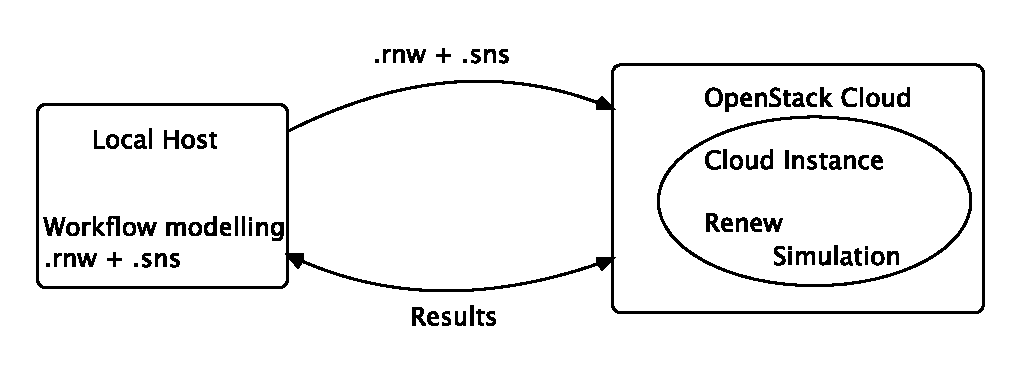
\includegraphics[width=0.7\textwidth]{openstacksimulation}
\caption{\Renew{} Simulation in the Cloud (from \cite{Bendoukha+15a})}
\label{fig:renew_cloud}
\end{figure}
%
 
Unfortunately, the current solution raises other interesting issues that need more investigation.
%
For example,  our proposition is based on the fact that workflows are executed once as a single process.
%
There is at the moment no mechanism to control the simulation of the workflow in the Cloud.
%
We mean by \emph{control}: the management of firing the Petri nets transitions in the Cloud instance. 
%
\Renew{} already provides the possibility to control the simulation by specific commands like: \emph{simulation run}, \emph{simulation halt} or \emph{simulation stop}.
%\footnote{More information about these commands can be found in \cite[p.106]{Kummer+13a}.}.  
%
Nevertheless, it is not possible to use these functionalities within a Cloud instance.
%
This should be in priori customized.
%
What about the ability to decompose the workflow in order enable selected execution of the tasks composing the workflow?
%
For this purpose we are investigating other alternatives as the remote execution of \Renew{}.
%
One of these solutions have been already discussed in \cite{Bendoukha+15a}.
%
In the latter work we provide mechanisms and implementation for moving the execution of computation- and time- consuming workflows into the Cloud.
%
Different kind of interfaces are provided to enable remote execution of \Renew{} in the Cloud.
%
These interfaces define how input and output to the Cloud calls are defined.
%
They range from simple, simulation and complex.

Interesting for the current work are the complex interfaces.
%
Through such kind of interface we seek bringing intelligence and autonomy to the managing system.
%
Concretely, special \emph{agents} are used as \emph{gateways} between the workflow (Petri net) model and the Cloud.
%
With respect to the \Mulan{}/\Capa{} framework, there exists a \emph{WebGateway Agent} \cite{Betz+14}.
%
It plays the role of a gateway between \Renew{} and the Web environment. 
%
Since Grass GIS commands can be also published as Web services (see Section.~\ref{sec:Cloudmigration}) coupling the WebGateway functionality into the architecture proposed in Section.~\ref{sec:Cloudmigration} will certainly enhance building agent-based scientific workflows.


